\subsection{Bubble \& Eat}

\subsubsection{Package}
Il package della demo Bubble \& eat è composto da due ulteriori packages: \Customer{} e ristorante. 
Il primo si riferisce soltanto all'utente \Customer{}. Il secondo invece contiene i package di tutti gli altri attori:
\begin{itemize}
	\item \Manager{};
	\item \Chef{};
	\item \Deliveryman{};
	\item \Purchasingmanager{}.
\end{itemize}
Nel package Restaurant, inoltre, è anche contenuto il pacchetto Order\-Gateway.\\
Lo scopo del package Order\-Gateway è quello di creare, modificare ed eliminare le ordinazioni interagendo con il database che le contiene.
Tutti gli attori interni ed esterni al ristorante hanno dipendenze verso l'Order\-Gateway.
%\begin{figure}[H]
%	\centering
%	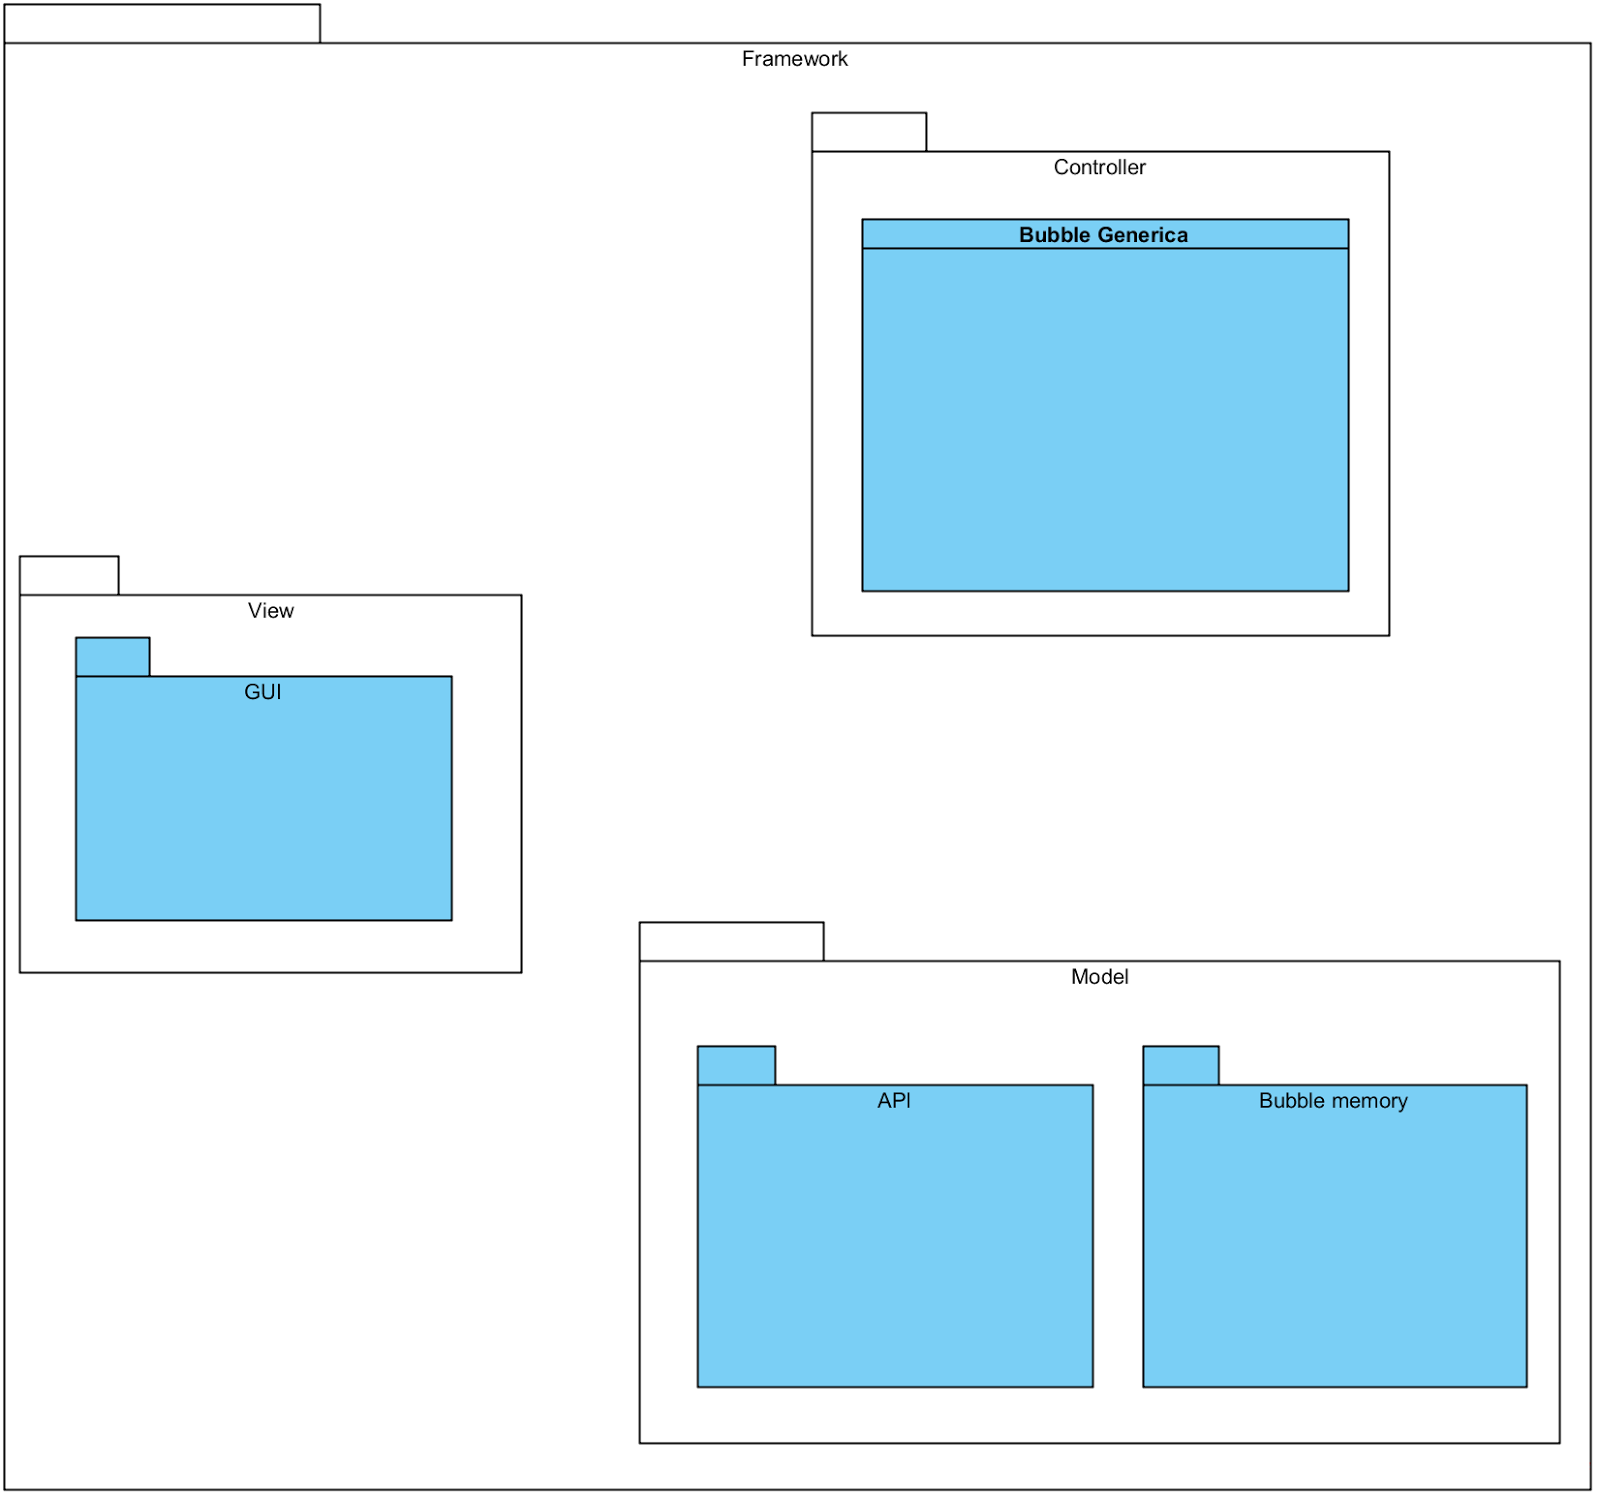
\includegraphics[width=14cm]{../../documenti/SpecificaTecnica/diagrammi_img/framework.png}
%	\caption{Demo Bubble \& Eat}
%\end{figure}

\subsubsection{Package Order\-Gateway}
Il package Order\-Gateway si occupa di gestire le interazioni tra attori e database e le eventuali comunicazioni tra gli stessi attori. Il package internamente è composto dalle classi Order\-Gateway e Menu e dal package Orders.\\
Il package Orders definisce le ordinazioni e la collezione di quest'ultime che verranno poi costruite seguendo il Factory method come design pattern dalla classe Menu.\\
Tutte le interazioni con gli elementi descritti sopra sono rese disponibili agli attori dalla classe Order\-Gateway.
%\begin{figure}[H]
%	\centering
%	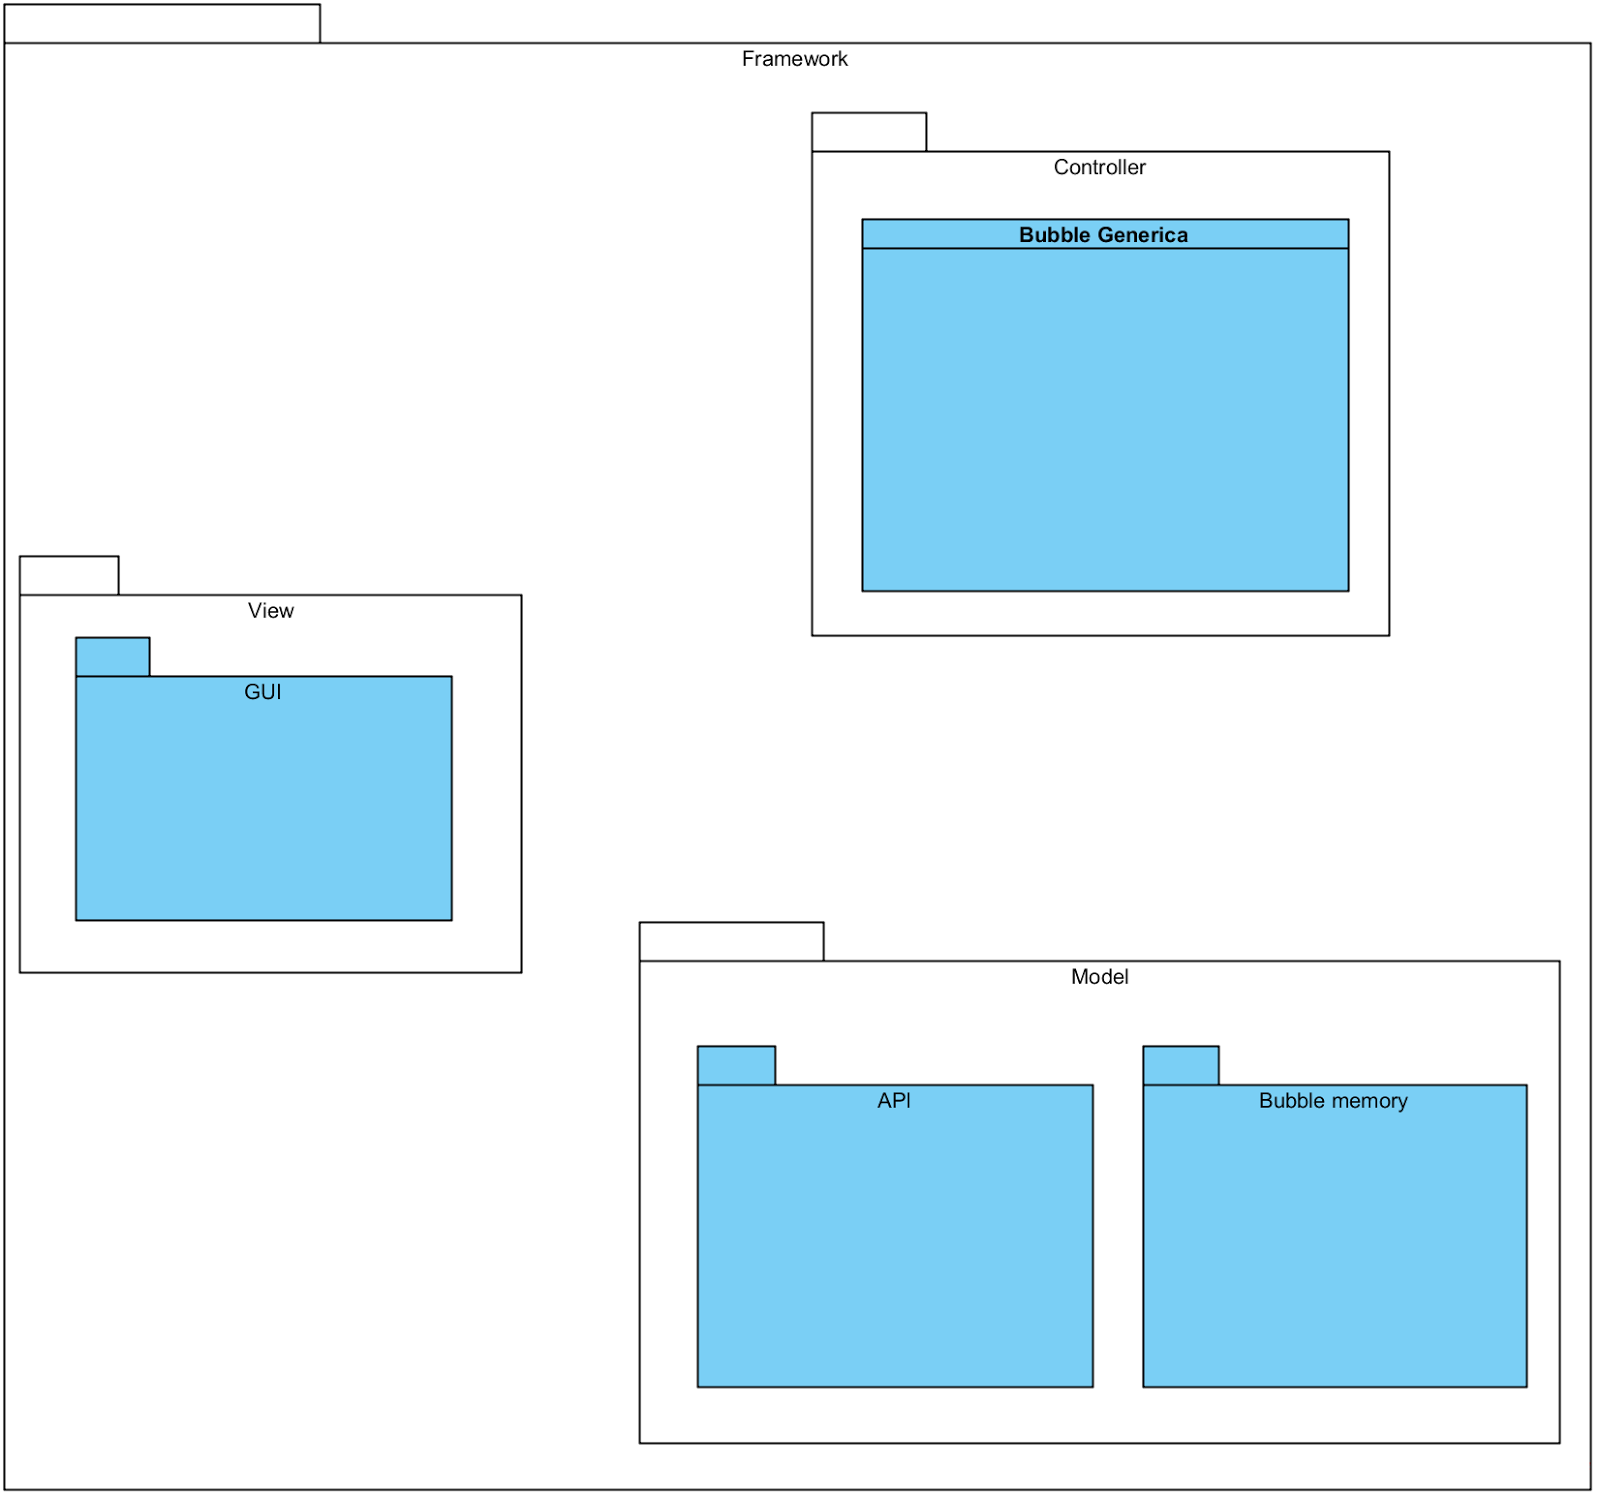
\includegraphics[width=14cm]{../../documenti/SpecificaTecnica/diagrammi_img/framework.png}
%	\caption{Package Order\-Gateway}
%\end{figure}

\subsubsection{Struttura delle classi}
%\begin{figure}[H]
%	\centering
%	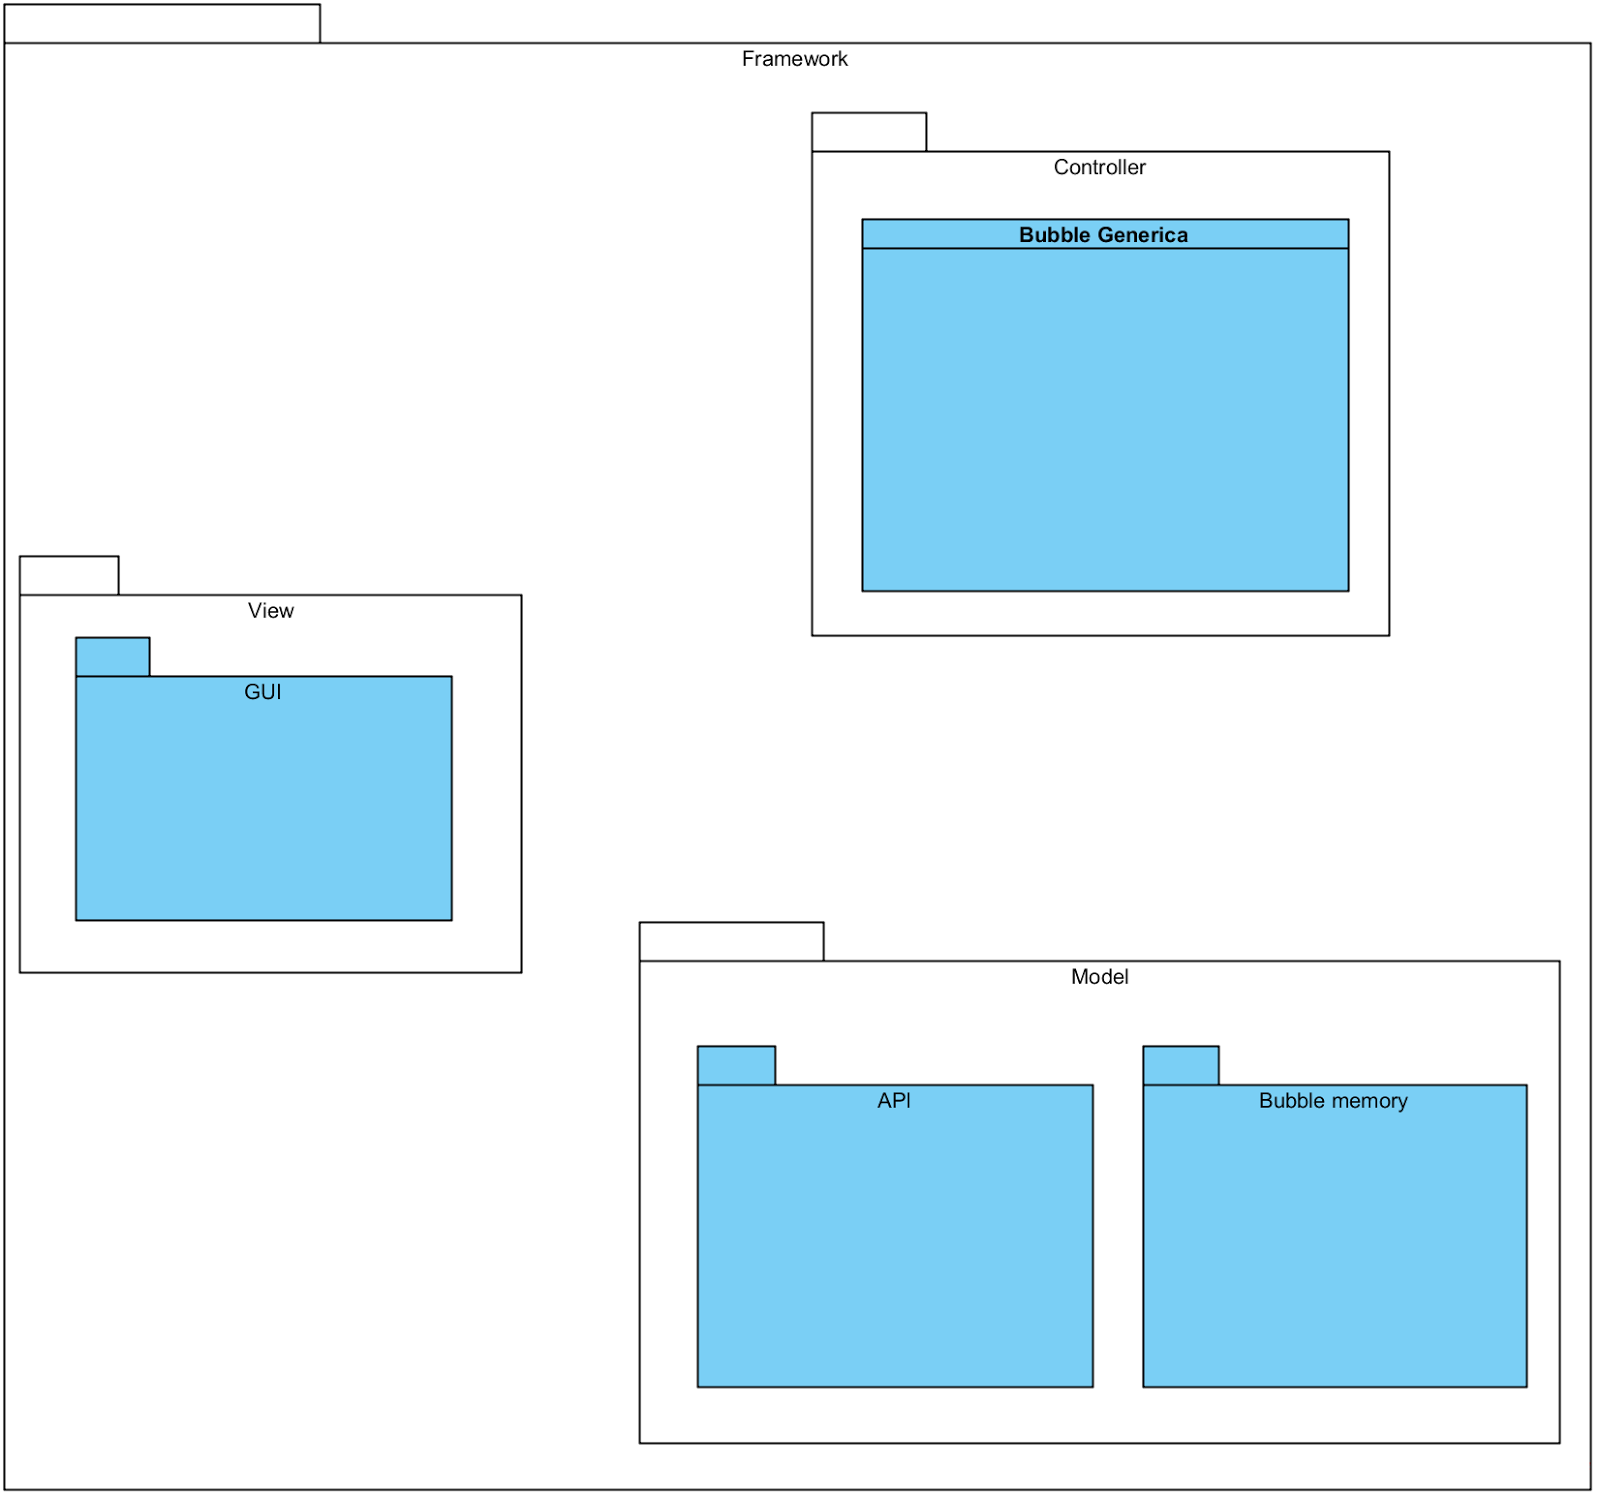
\includegraphics[width=14cm]{../../documenti/SpecificaTecnica/diagrammi_img/framework.png}
%	\caption{Diagramma di struttura delle classi}
%\end{figure}

\subsubsection{Descrizione classi}

\paragraph{DemoBubble\&eat\-::Customer\-::Bubble\-Customer}\label{eat-customer}\mbox{}\\
\textbf{Descrizione:}\\
La classe permette al \Customer{} di consultare il menu, registrare i propri dati personali e inviare le proprie ordinazioni.\\
\textbf{Utilizzo:}\\
Questa classe attraverso l'Order\-Gateway riceve il menu da consultare per mezzo del quale può creare la propria ordinazione.\\

\paragraph{Demo\-Bubble\&eat\-::Restaurant\-::Manager\-::Bubble\-Manager}\label{eat-manager}\mbox{}\\
\textbf{Descrizione:}\\
La classe permette al \Manager{} di gestire il menu, il magazzino e le ordinazioni.\\
\textbf{Utilizzo:}\\
Questa classe permette di gestire tutte le operazioni fornite da Order\-Gateway ed ha la possibilità di manipolare il magazzino e le ordinazioni.\\

\paragraph{Demo\-Bubble\&eat\-::Restaurant\-::Chef\-::Bubble\-Chef}\label{eat-chef}\mbox{}\\
\textbf{Descrizione:}\\
La classe permette allo \Chef{} di consultare le ordinazioni e di impostare lo stato di una ordinazione in modo da renderla disponibile alla consegna.\\
\textbf{Utilizzo:}\\
Questa classe attraverso l'Order\-Gateway recupera e visualizza le ordinazioni e offre la possibilità allo \Chef{} di modificarne lo stato.\\

\paragraph{Demo\-Bubble\&eat\-::Restaurant\-::Deliveryman\-::Bubble\-Deliveryman}\label{eat-deliveryman}\mbox{}\\
\textbf{Descrizione:}\\
La classe permette al \Deliveryman{} di consultare gli ordini pronti alla consegna, di ottenere i dati personali dei \Customer[2]{} relativi alle consegne selezionate e di eliminarle una volta completate.\\
\textbf{Utilizzo:}\\
Questa classe attraverso l'Order\-Gateway riceve la lista delle ordinazioni da consegnare, le visualizza e permette di selezionare le consegne ed eliminarle una volta selezionate.

\paragraph{Demo\-Bubble\&eat\-::Restaurant\-::PurchasingManager\-::Bubble\-Purchasing\-Manager}\label{eat-purchasing}\mbox{}\\
\textbf{Descrizione:}\\
La classe permette al \Purchasingmanager{} di recuperare e visualizzare la lista della fornitura da acquistare oltre ad eliminare gli acquisti dalla lista.\\
\textbf{Utilizzo:}\\
Questa classe recupera dall'Order\-Gateway la lista degli acquisti, la visualizza e consente di eliminare gli acquisti presenti nella stessa.

\paragraph{Demo\-Bubble\&eat\-::Restaurant\-::Order\-Gateway\-::Order\-Gateway}\label{eat-gateway}\mbox{}\\
\textbf{Descrizione:}\\
La classe permette a tutti gli attori di interagire con il database attraverso apposite funzioni e si occupa di gestire le interazioni con il menu e l'insieme delle ordinazioni contenute nell'OrderContainer. La classe si occupa inoltre di inviare le notifiche agli attori quando viene richiesto o in maniera automatica ed aggiorna le risorse e le liste in tempo reale.\\
\textbf{Utilizzo:}\\
Questa classe offre diverse funzionalità agli attori per manipolare il database, le ordinazioni contenute nell'OrderContainer ed il menu, che permette a sua volta la creazione delle ordinazioni. Queste funzioni saranno disponibili o meno a seconda del tipo di attore.\\
La classe aggiorna le risorse in modo automatico scalando gli ingredienti dai valori impostati per ogni piatto nel menu. Ha inoltre delle funzioni di notifica che possono essere impostate automaticamente durante le operazioni o chiamate da alcuni attori.

\paragraph{Demo\-Bubble\&eat\-::Restaurant\-::Order\-Gateway\-::Menu}\label{eat-menu}\mbox{}\\
\textbf{Descrizione:}\\
La classe permette la creazione delle ordinazioni ed attraverso l'Order\-Gateway fornisce diverse operazioni agli utenti:
\begin{itemize}
	\item \Customer{}: recupero del menu e creazione dell'ordinazione;
	\item \Manager{}: recupero e modifica del menu.
\end{itemize}
\textbf{Utilizzo:}\\
Questa classe implementa il design pattern del Factory method e permette la creazione delle orinazioni, inoltre fornisce dei metodi per modificare ed ottenere il menu.

\paragraph{Demo\-Bubble\&eat\-::Restaurant\-::Order\-Gateway\-::Order\-::Order}\label{eat-order}\mbox{}\\ 
\textbf{Descrizione:}\\
Questa classe definisce il contenuto dell'ordinazione. Contiene gli elementi scelti dal menu e i dati forniti dall'utente per la consegna.\\
L'ordinazione è definita anche da uno stato e la classe offre i metodi per modificarlo. \\
\textbf{Utilizzo:}\\
Questa classe permette di inserire gli elementi del menu nell'ordinazione e di modificare lo stato della stessa. 

\paragraph{Demo\-Bubble\&eat\-::Restaurant\-::Order\-Gateway\-::Order\-::Order\-Container}\label{eat-container}\mbox{}\\
\textbf{Descrizione:}\\
La classe permette la gestione di una collezione di ordinazioni definiti dalla classe Order.\\
\textbf{Utilizzo:}\\
Questa classe offre la possibilità di aggiungere, rimuovere e restituire elementi da una collezione di ordinazioni.